The multiplicative algebraic reconstruction technique (MART) was developed for limited-angle tomography problems, in which a small number of projections are used to reconstruct a volume \citep{Okamoto1991,Verhoeven1993}. 
As ESIS has only four projections through the $(x,y,\lambda)$ volume, it is a good candidate for this approach.
When testing a variety of inversion methods on MOSES data, \citet{Fox2011} identified MART as most promising of several methods in terms of speed and fidelity.
\citet{Rust2017} applied a slightly different version of MART to the MOSES data paired with a wavelet based partial reconstruction technique for better background subtraction and event isolation.
Due to its speed, simplicity, and automatic enforcement of image positivity we have chosen MART for our first inversion of Level 3 ESIS data.


With MART we seek to reconstruct the true spatial-spectral cube, $I_{xy\lambda}$, using all four ESIS images from a single exposure.
Each ESIS image, $i_{\theta x'y'}$, can be expressed as an angled projection through $I_{xy\lambda}$ onto a 2-D detector, or,
\begin{equation}
i_{\theta x'y'} = \sum_\lambda I_{\theta x'(y'-\delta\lambda)\lambda},
\end{equation}
where
\begin{equation}
I_{\theta x'y'\lambda} = \mathcal{R}_\lambda(\theta)\,I_{xy\lambda},
\end{equation} 
and, $\mathcal{R}_\lambda (\theta)$, is a rotation about the $\lambda$ axis into the primed detector coordinates $[x',y']$. 
In this rotated system, $y'$ is the dispersion direction.
There is one ESIS image for each $\theta \in \left\{ -67.5^{\circ}, -22.5^{\circ}, 22.5^{\circ},67.5^{\circ} \right\}$, representing the  orientations of each ESIS channel.
Projections through $I$ are done along lines of constant $y'-\delta\lambda$.
For our specific implementation, the resolution of $I_{xy\lambda}$ in $\lambda$ is chosen to be 28\,m\AA\,pix$^{-1}$, the spectral dispersion of an ESIS grating, such that $\delta = 1$. 

MART attempts to find the true spatial spectral cube $I_{xy\lambda}$ by iteratively correcting a guess cube, $G_{xy\lambda}$, until its projected images, $g_{\theta x'y'}$, match each ESIS image, $i_{\theta x'y'}$, with a reduced chi-squared, $\chi_{R,\theta}^2$,  less than one.
Our procedure is as follows:
\begin{enumerate}
	\item \label{step:guess} Create a guess cube,
	initialized as 
	$G_{xy\lambda} = 1$ on the same domain as $I$. 
	\item \label{step:contrast} Enhance the contrast of $G$ and normalize. 
	\begin{equation}
	G \leftarrow \frac{G+G^{(1+\Psi)}}{\sum_{xy\lambda}G+G^{(1+\Psi)}}\sum_{xy\lambda}G, 
	\end{equation}
	
	\item \label{step:smooth} Convolve $G$ with smoothing kernel $K$, $G \leftarrow G * K$,
	in our case,
	\begin{equation}
	\label{eq:kernel}
	K_{ijk} = \frac{2^{3-|i|-|j|-|k|}}{64} \quad \text{for}\quad i,j,k = -1,0,1.
	\end{equation}
	\item \label{step:project} Assuming $\delta=1$, sum $G_{\theta x'y'\lambda}$ along lines of constant $y'-\lambda$ to calculate a projection for each angle $\theta$,
	\begin{equation}
	g_{\theta x'y'} = \sum_\lambda G_{\theta x'(y'-\lambda)\lambda}, 
	\end{equation}
	where
	\begin{equation}
	G_{\theta x'y'\lambda} = \mathcal{R}_\lambda(\theta)\,G_{xy\lambda},
	\end{equation} 
	and, $\mathcal{R}_\lambda (\theta)$, is a rotation about the $\lambda$ axis. 	
	
	\item \label{step:chisquared} Calculate reduced chi-squared and check for each channel for convergence, in this case that $\chi_{R,\theta}^2 < 1$ , 
	\begin{equation}
	\chi_{R,\theta}^2 = \frac{1}{N_{x'} N_{y'}}\sum_{x'y'} \frac{(i_{\theta x'y'}-g_{\theta x'y'})^2}{g_{\theta x'y'}+\sigma^2_{RN}},
	\end{equation}
	where $\sigma_{RN}$ is the read noise in photons, $N_{x'}$ is the total number of elements along $x'$.
	
	\item Calculate correction factors for each unconverged channel, $\theta_{uc}$, weighted by $\gamma$, 
	\begin{equation} \label{eq:correctionfactor}
	c_{\theta x'y'} = \left[\frac{g_{\theta x'y'}}{i_{\theta x'y'}}\right]^\gamma,
	\end{equation}
	where $\gamma = 2/n$ with $n$ equal to the total number of channels.
	
	\item Assign correction factors to lines of constant $y'-\lambda$ in the volume $(x',y',\lambda)$,
	\begin{equation}
	C_{\theta x'(y'-\lambda)\lambda} = c_{\theta x'y'}
	\end{equation}	
	\item \label{step:correct} Apply a weighted product of each derotated correction to $G$ ,
	\begin{equation}\label{eq:correct}
	G \leftarrow G\left\lbrace  \,\prod_{\theta\in\Theta_{\mathrm{uc}}}  \mathcal{R}_\lambda(-\theta)C_{\theta x'y'\lambda} \right\rbrace^{1/m_{\mathrm{uc}}},
	\end{equation}
	where $m_{\mathrm{uc}}$ is the total number of unconverged channels and $\Theta_{\mathrm{uc}}$ denotes the set of unconverged channels.
	
	\item Repeat steps \ref{MART}\ref{step:project}-\ref{MART}\ref{step:correct}
	until every channel has converged at step \ref{MART}\ref{step:chisquared}. Once converged proceed to next step.
	\item Return to Step \ref{MART}\ref{step:contrast} if additional filtering is desired.
\end{enumerate}
The above algorithm begins with an arbitrary, flat guess (step \ref{MART}\ref{step:guess}). The guess is rapidly modified to fit the data projections $i_{\theta x' y'}$ by steps \ref{MART}\ref{step:project}-\ref{MART}\ref{step:correct}, which project through the guess, compare the results to the data, calculate and apply intrinsically positive correction factors. 
When applied to  ESIS Level 3 data the total number of channels is $n = 4$. 
The rotations $\mathcal{R}_{\lambda}(\pm{\theta})$ cause ringing due to the Gibbs phenomenon associated with resampling and interpolation. 
All negative values resulting from this ringing are set to zero.
In our case, the ringing occurs mostly at the sharp discontinuity at the edge of the field stop octagon. 

\begin{figure}[htb!]
	\center
	\resizebox{!}{7.2in}{
		\begin{tikzpicture}
		%begin by adding a node for each figure
		\node[inner sep=0pt] (imgs) at (0,0)
		{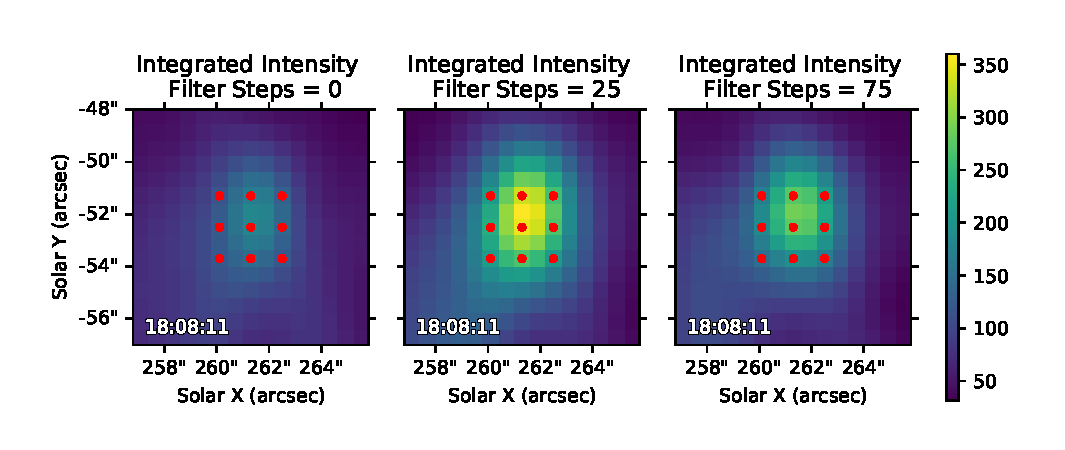
\includegraphics[]{perfectx_invert_comp_a}};
		\node[inner sep=0pt] (lps) at (0,-9.5)
		{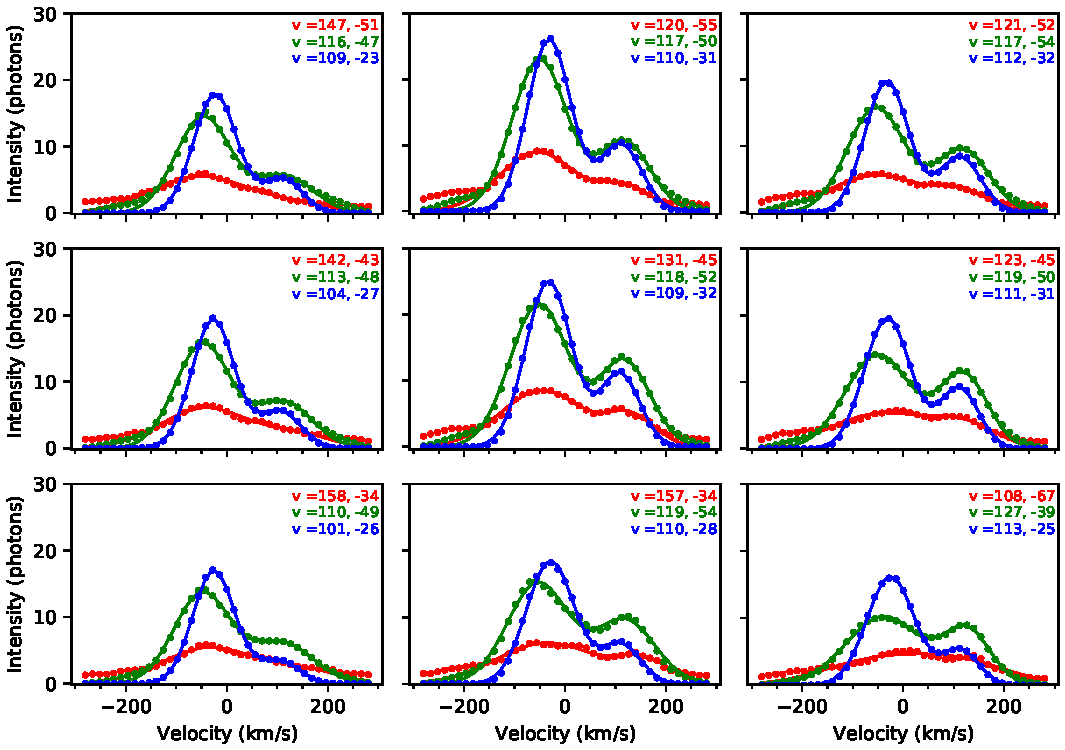
\includegraphics[]{perfectx_invert_comp_b}};
		\end{tikzpicture}
	}
	\caption{Comparison of MART outputs for a single timestamp in Event c (Figure \ref{fig:l3_dif} and \ref{fig:perfect_x_inverted}) with different amounts of filtering. 
		The top row shows the total inverted intensity at a single timestamp each using a different number of MART filtering steps (steps \ref{MART}\ref{step:contrast} and \ref{MART}\ref{step:smooth}).  
		The lower grid shows the inverted O\,\textsc{v} spectral line at each red dot for 0, 25, and 75 filtering steps in red, green, and blue respectively.}
	\label{fig:perfect_x_invertcomp}
\end{figure}


The inversion is ill-posed, in the sense that multiple different $G_{xy\lambda}$ cubes can satisfy $\chi_{R,\theta}^2<1$. 
In particular, tomographic inversion algorithms such as MART tend to smear intensity along the projection directions \citep{KakSlaney2001}. 
This tendency is especially strong when there are only a few projections. 
This smearing results in rapid convergence to an intensity distribution in the volume that matches the projection data, but results in artificial streaks that intersect and produce anomalous bright sources. 
Since the resulting artifact forms a gridlike pattern of enhancements, we use the nickname ``plaid'' to describe it. 
In the reconstructed ESIS data cube, the plaid artificially enhances the wings of the spectral line wherever projections through unrelated intense sources happen to meet. 
To suppress the plaid, we implement an outer filtering loop that enhances the contrast of $G_{xy\lambda}$ and applies smoothing prior to the MART corrections to further constrain our inversions. 
The contrast enhancement (step \ref{MART}\ref{step:contrast}) works to suppress the intensity of the artifacts and redistribute their intensity into the brightest features. 
We aim thereby to arrive at a solution with the fewest sources that are consistent with the appearance of the data. 
By itself, the contrast enhancement can tend to develop excess power at the Nyquist frequency and (sometimes) numerical instability. 
These undesired effects of contrast enhancement are suppressed by a smoothing filter (step \ref{MART}\ref{step:smooth}).

As a result of the plaid suppression technique described above, our implementation of MART has two free parameters, namely the contrast enhancement exponent $\Psi$ and the number of times the filtering step (steps \ref{MART}\ref{step:contrast} and \ref{MART}\ref{step:smooth}) is applied.
In order to better understand the impact of these two parameters on our inversions we inverted a single exposure of Event c (Figure \ref{fig:l3_dif} and \ref{fig:perfect_x_inverted}) using several different values of each free parameter.
During this exercise we found that lowering $\Psi$ resulted in faster MART convergence, but required more applications of the filtering step to minimize the plaid.
Increasing $\Psi$ lowered the number of required filtering loops, but increased the convergence time of each MART iteration and quickly led to overfiltered and artificial looking results.
For smaller values of $\Psi$, less than approximately .4, we find $\Psi$ to be nearly degenerate with the number of filtering steps, i.e. inversions found using a lower $\Psi$ and more filtering steps are similar to those found using a higher $\Psi$ and less filtering steps.
In the end we chose to use $\Psi=0.2$ in an effort to not overfilter our inversions and maintain a reasonable total algorithm convergence time. 

Figure \ref{fig:perfect_x_invertcomp} shows the results of changing the total number of filtering steps with $\Psi=0.2$.
While other numbers of filtering steps were tried, the inverted results after 0, 25, and 75 steps sufficiently illustrate the effect of varying this parameter. 
The impact of plaid is most evident in the red spectral lines in Figure \ref{fig:perfect_x_invertcomp}, where the contrast enhancement filter wasn't used at all.
Despite excess intensity in the wings of the lines from excessive plaid, the brightest pixels are still double peaked in nature and the two Gaussian fits reasonably approximate the inverted line profiles.
The blue spectral lines in Figure \ref{fig:perfect_x_invertcomp} correspond to 75 filtering steps, after which point the filtering has converged, in the sense that further filtering iterations have no effect.
Since the contrast enhancement filter is designed to pull intensity from the background and into regions of stronger signal, it has the effect of clumping the intensity into a smaller area.
This causes much less intensity in the far wings of the line profile and narrower peaks overall.  
Unfortunately this also has the ill effect of clumping background intensity where there is very little signal.
In low signal regions where we would expect a relatively flat, low intensity, and noisy line profile overfiltering can cause what little intensity is there to clump together artificially far out in the wings of the line.
Therefore we choose to compromise and run the filtering step enough times, in our case 25, such that the majority of the artificial intensity in the wings has been beaten down, but not so much that we artificially remove a flat noisy line profile in low signal regions. 

Regardless of the parameters chosen, we find that our inverted results match qualitative interpretations of ESIS difference images.
The degree of filtering affects the breadth of the individual Gaussian components, so that they are more or less resolved. 
Their velocities and relative intensities also vary, but are less affected. 
An extreme parameter range was explored, from no filtering to maximal (fully converged) filtering. 
We have argued that both extremes represent implausible solutions on physical grounds. Consequently, we conclude that the relative velocities and intensities of the double Gaussian fits are robust, while their widths are uncertain. 

The final configuration we used when inverting all Level 3 data used 25 filtering steps and a contrast enhancement exponent of $\Psi=0.2$.
In this configuration, a single exposure of a small region like event c (with final inverted dimensions of $[x,y,\lambda] = [140,140,41]$\,pixels) can be inverted in $\sim$75\,seconds on a single thread of a four core 2.8\,GHz processor.
Since the inversion of each ESIS exposure is independent, inversions can be done on multiple threads to increase efficiency when inverting additional exposures.